\section{Allocation of time and resources}
This section presents an overview of the time and resource allocation in the project.

\subsection{Time allocation}
At the beginning of the project, the team did an estimation on how much time we would spend on each part of the project. In figure~\ref{fig:piechart} we show an overview on how much time we actually spent.

\begin{figure}[H]
\centering
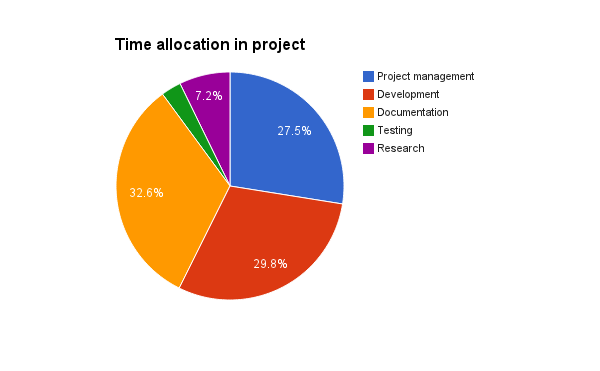
\includegraphics[width=0.6\textwidth, clip, trim=4cm 2cm 4cm 1cm]{ch/retrospect/fig/timePie.png}
\caption{Pie chart of time spent on different parts of the project.}
\label{fig:piechart}
\end{figure}

When comparing the actual time spent with the estimated time from table~\ref{tab:timeEstWP}, we see that the team spent more time on \todo{add more here when illustrations are ready. Sprint 8 on release chart is estimated time used.}

\begin{figure}[H]
\centering
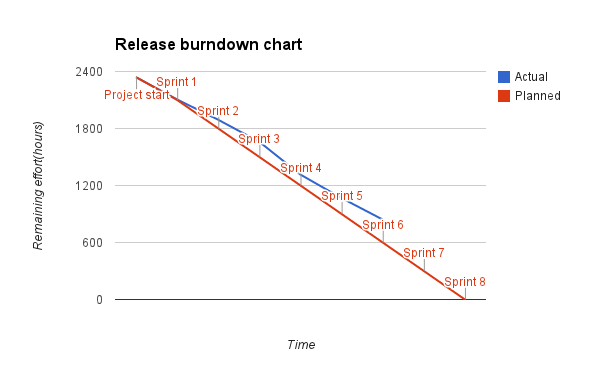
\includegraphics[width=0.7\textwidth, clip, trim=1.1cm 0.5cm 1.2cm 1cm]{ch/retrospect/fig/release.png}
\caption{Project release burn down chart}
\label{fig:release}
\end{figure}

\noindent In the release burn down chart, displayed in figure~\ref{fig:release}, we compare the estimated project progress with the progress we actually made. As the graph shows, the team worked less than the estimated number of hours. There are several reasons for this, including unplanned absence of team members, underestimation of tasks and too heavy workload due to deliveries in other classes. Another large factor in the discrepancy between the planned hours and the actual time spent is the manner of which work hours are logged. The hours logged in Yodiz, which are shown in figure~\ref{fig:release}, only represent how long specific tasks took to complete. The logging done in Yodiz is used primarily to estimate user stories and tasks, and not to log precise work hours. This gives a deviation in hours spent and hours logged, which in time amounts to a notable amount. Fortunately, the team had deliberately overestimated the number of work hours to compensate for lost time due to the school trip to China. This action resulted in that the team still was able to fulfil the course requirement and complete the assignment within the project's time scope.

\todo{oppdatere release og pie charten når sprint 8 er ferdig skrevet}

\subsection{Resource allocation}
As described in section~\ref{sec:availResources}, the team had several resources available, including a supervisor, the customer and, of course, the other team members. The team had internal meetings at least two times a week, and also an eight hour work session once a week. In addition, we had weekly meetings with the customer and meetings with the supervisor every other week.

To have meetings at such regular times has been of great value for the team. It saved a lot of time to have pre-booked meeting rooms, and it was also easier for the parties involved in the project to prepare for the meetings.

During the meetings with the supervisor, we were given valuable input and feedback regarding customer relations, and the content and structure of the report. Although the role of the supervisor was unclear to the team early on, we quickly learned that he was more of a guide we could use to help us, and not a supervisor that was in place to make sure we did our work. The only real oversight the supervisor had was the activity report which included a work log and a summary of the progress made since the last meeting.

Communicating with the customer on a regular basis has reduced the probability of misunderstandings arising and increased the likelihood that the team would deliver a product the customer would be greatly satisfied with. 

One of our valuable decisions in this project has been to actually have fixed meeting times, assuring that the entire team would be kept updated and involved. On these internal meetings, the team planned and distributed tasks among the team members, and discussed occurring issues. We also had assigned each team member an area of responsibility, so that no important parts of the project would be neglected, but also as a way to keep the motivation high and further involve the team members.